%!TEX root = ../paper.tex

\section{Smart Restaurant Experience}
\label{sec:smart_restaurant_experience}
% Normal restaurant experience
% Smart restaurant experience
% For waiters
% For customers
% Figures: Smart restaurant from wiki
% -> Screenshots?

Since we aim to improve restaurants' service, we need to compare our approach
with what usually happens. ??
Usually, the customer arrives at the restaurant, get a sit and calls a waiter
to place his order. However, the waiter can be busy processing orders
from other customers, which can delay this new order.
Figure~\ref{fig:smart_restaurant} shows the interactions between the
customer and the waiter in a normal restaurant (on the left) and in
a smart restaurtant (on the right). It is possible to see that our
solution removes some interactions. For instance, the customer does not
need to wait until he is able to place his order.
The main goal is not to replace the workers but instead help them to do a
better job.
There are three groups of users of the solution being proposed here:

\begin{description}
  \item[Waiters] who will use a web application to see the customers'
  orders;
  \item[Owners] who will use a mobile app to configure the
  restaurants' menu and the mapping between the tables and the beacons;
  \item[Customers] who will use a mobile app (not the same app as the
  Owners use) that will notify him when he arrives at the restaurant and
  will present the menu.
\end{description}

Next, for each kind of user, we will present the main features and their
advantages.

\begin{figure}[!ht]
  \centering
    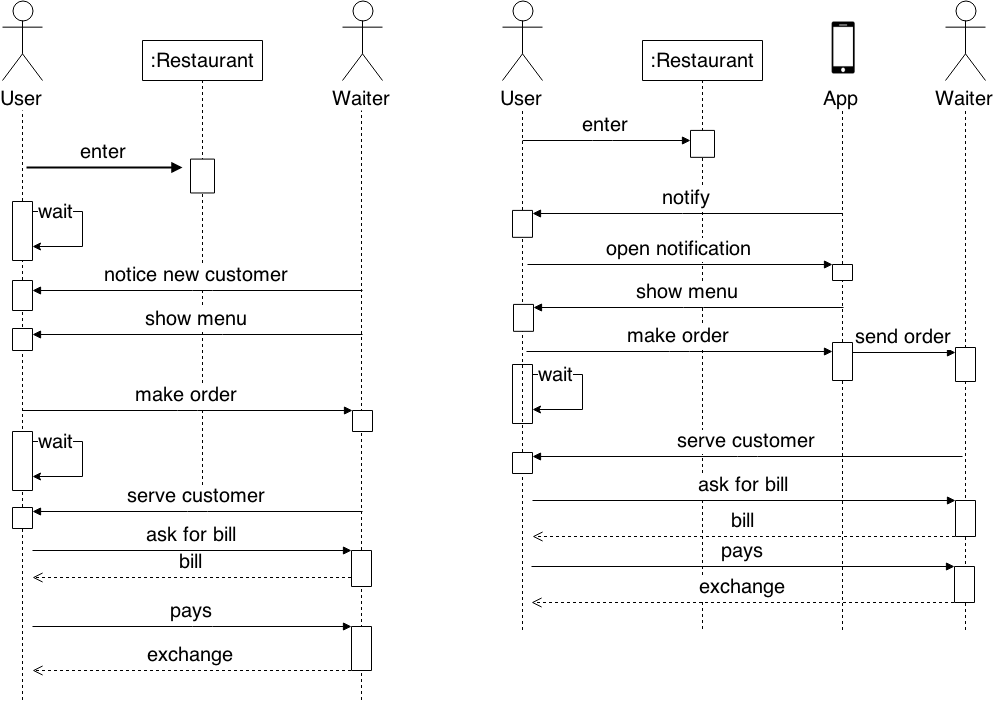
\includegraphics[width=1\textwidth]{figures/smart-restaurant}
    \caption{Sequence diagram showing the interactions between
    the customer and the waiter in a normal restaurant (on the left)
    and in a Smart Restaurant(on the right)}
    \label{fig:smart_restaurant}
\end{figure}

\subsection{Waiters}
\label{sub:waiters}
% Features
%
This group of users is responsible for processing the customers' orders.


\subsection{Owners}
\label{sub:owners}

\subsection{Customers}
\label{sub:customers}
As it is shown in figure~\ref{fig:smart_restaurant} some interactions between
the customer and the waiter can be replaced by a mobile app.
For this group of users, the main feature is to allow them to place
the orders using their smartphones. The mobile app detects in which table
the customer is in and sends that information to the web application that the
Owners use. When the customer places his order, he does not need to type
the number of the table. This way, the customer will get his orders
processed faster.
